\section{Testscenario}

Her følger en beskrivelse av webapplikasjonen migrasjon med DBUpgradinator blir testet på. Nettbutikken ''WebShop'' benytter nøkkelverdi\-lageret Project Voldemort for å lagre et register over dens kunder. Kundene bor stort sett enten i Storbritannia eller i Australia. Aggregatene som lagres av Voldemort er flate og består av strengnøkler og strengverdier.

\begin{figure}[hbtp]
    \centering
    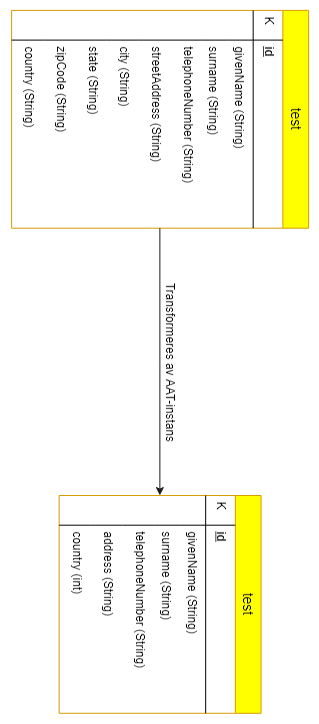
\includegraphics[scale=0.8]{fig/WSS-AggregatModell.png}
    \caption{Datamodeller for aggregatene til skjemaversjon ''x'' og dets etterfølger, ''y''.}
    \label{fig11}
\end{figure}

I skjemaversion ''x'' har aggregatene til WebShop følgende attributter: \texttt{givenName} (fornavn), \texttt{surName} (etternavn), \texttt{telephoneNumber} (telefonnummer), \texttt{streetAddress}, \texttt{city} (byaddresse), \texttt{state} (delstat - for australske og eventuelt amerikanske kunder), \texttt{zipCode} (postkode, hvis system varierer fra land til land), og \texttt{country} (landet til addressen).
